\documentclass[11pt]{article}

% Change "review" to "final" to generate the final (sometimes called camera-ready) version.
% Change to "preprint" to generate a non-anonymous version with page numbers.
\usepackage[review]{acl}

\usepackage{times}
\usepackage{latexsym}
\usepackage[T1]{fontenc}
\usepackage[utf8]{inputenc}
\usepackage{microtype}
\usepackage{inconsolata}
\usepackage{graphicx}
\usepackage{booktabs}
\usepackage{amsmath,amssymb}
\usepackage{tikz}
\usetikzlibrary{arrows.meta,positioning,fit}

\title{The Latent Relay is a Prefix, Not a Message:\\
Interpreting Inter-Agent KV Communication}

\author{First Author \\
  Affiliation / Address line 1 \\
  Affiliation / Address line 2 \\
  \texttt{email@domain} \\\And
  Second Author \\
  Affiliation / Address line 1 \\
  Affiliation / Address line 2 \\
  \texttt{email@domain} \\}

\begin{document}
\maketitle
\begin{abstract}
Latent multi-agent systems such as LatentMAS replace text messages with a
shared key--value (KV) cache: silent Planner, Critic, and Refiner agents grow
a relay of latent steps, and only a Judger decodes. The design is motivated by
the claim that this relay is a \emph{richer native communication channel} than
language. We treat that claim as an interpretability question and intervene on
the cache after the upstream agents finish.

Two complementary tests argue that the $K{=}40$ tape is mostly a
content-insensitive prefix. \emph{Swap:} a wrong-item cache matches a
right-item cache for Judger accuracy under matched token budgets.
\emph{Delete:} after a full $K{=}40$ rollout, keeping attention sinks plus a
small top-$\|K\|$ subset of slots leaves GSM8K and MATH-500 accuracy in the
same band as the uncompressed system (96.3\% vs.\ 95.7\%; 85.7\% vs.\ 83.7\%,
three seeds, paper sampling). Aggressive deletion (keep-16) does not collapse
GSM8K accuracy but makes the Judger longer, so a little structure must remain.
Eviction is not a competing multi-agent algorithm and is not a substitute for
running fewer latent steps; it is a length ablation of a \emph{finished}
$K{=}40$ cache. The systems side-effect is smaller Judger prefixes and lower
batched KV memory, not skipped upstream compute.

We recommend reading LatentMAS's native channel as a decoding-mode scaffold,
not as an instance-specific message.
\end{abstract}

\section{Introduction}
\label{sec:intro}

Multi-agent prompting lets models play specialized roles and exchange
text~\citep{du2023society,wu2023autogen,wei2022cot}.
\citet{zou2025latentmas} push the messages \emph{inside} the transformer:
three upstream agents run a fixed number $K$ of latent forward passes,
emit no tokens, and append to a shared KV cache
(\texttt{past\_key\_values}). A final Judger attends to that cache and
generates the answer. They argue that this \emph{latent collaboration} is
richer than language and, in their main tables, operate at a moderate latent
budget on the order of $K{=}40$.

If the relay were an instance-specific reasoning transcript, two things should
fail. Replacing it with another problem's cache should hurt. Deleting most of
its slots after a long rollout should hurt. We find the opposite on the
settings we can measure carefully.

\paragraph{What this paper is.}
An analysis of the latent channel in a verified sequential LatentMAS
fork (Qwen3-14B; \citealp{qwen3}).
Contribution type: model analysis, not a new multi-agent method.

\paragraph{What this paper is not.}
We do not claim a compressor that beats LatentMAS on accuracy or
end-to-end latency. We do not claim that LatentMAS's latent-step sweep
(their reported peak near $K{\in}[40,80]$) is false: we did not rerun that
full grid. We do not claim that running $K{=}10$ is the same algorithm as
compressing a $K{=}40$ cache (\S\ref{sec:notk10}).

\paragraph{Interventions.}
(i)~Cache \emph{swap}: decode the Judger from another item's relay.
(ii)~Cache \emph{eviction}: after the same $K{=}40$ upstream pass, keep a
few sink positions plus the largest key-norm slots and decode.
Swap tests \emph{content}. Eviction tests \emph{length} of an already-built
tape. Together they support a simple picture: the native channel is a long,
noisy prefix that puts the Judger into a working decoding mode; it is not a
tight code for the answer.

\section{LatentMAS, in the form we study}
\label{sec:setup}

\paragraph{Pipeline.}
Sequential LatentMAS runs three silent agents then a text Judger:
$\mathrm{Planner}_K \to \mathrm{Critic}_K \to \mathrm{Refiner}_K$
grow a shared relay $C$, and only the Judger decodes.
Each silent agent realigns its last-layer state with $W_a$ and runs $K$
extra forwards, appending KV slots.
Figure~\ref{fig:pipe} marks the intervention: \emph{after} $C$ exists.

\begin{figure}[t]
\centering
\resizebox{\columnwidth}{!}{%
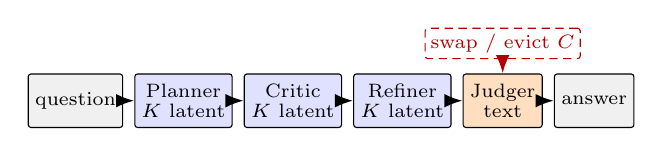
\begin{tikzpicture}[
  font=\scriptsize,
  box/.style={draw, rounded corners=1pt, align=center, inner sep=2.5pt, minimum height=0.68cm},
  arr/.style={-{Latex}, thick}
]
\node[box, fill=black!6] (q) {question};
\node[box, fill=blue!12, right=0.14cm of q] (p) {Planner\\[-1pt]$K$ latent};
\node[box, fill=blue!12, right=0.14cm of p] (c) {Critic\\[-1pt]$K$ latent};
\node[box, fill=blue!12, right=0.14cm of c] (r) {Refiner\\[-1pt]$K$ latent};
\node[box, fill=orange!25, right=0.14cm of r] (j) {Judger\\[-1pt]text};
\node[box, fill=black!6, right=0.14cm of j] (a) {answer};
\draw[arr] (q) -- (p);
\draw[arr] (p) -- (c);
\draw[arr] (c) -- (r);
\draw[arr] (r) -- (j);
\draw[arr] (j) -- (a);
\node[draw, densely dashed, red!70!black, rounded corners=1pt, inner sep=2pt,
      above=0.18cm of j, font=\scriptsize] (int) {swap / evict $C$};
\draw[arr, red!70!black] (int) -- (j);
\end{tikzpicture}%
}
\caption{Sequential LatentMAS. Silent agents grow a shared KV relay $C$;
only the Judger decodes. We intervene on $C$ immediately before Judger
decode.}
\label{fig:pipe}
\end{figure}

\paragraph{Fork.}
Code is a byte-for-byte copy of
\texttt{Gen-Verse/LatentMAS} at commit \texttt{9a9e4d3} (24/24 file SHAs).
At $K{=}40$, sequential HF decode, Qwen3-14B, a one-seed $n{=}150$ check
sits within $1$--$2.5$ points of their published GSM8K / ARC-Challenge /
MedQA table means (Appendix~\ref{app:fork}). Eviction is layered on that
path: we do not reimplement the agents.

\paragraph{Default operating point.}
Unless noted, $K{=}40$, Judger temperature $0.6$ and top-$p$ $0.95$
(their sampling), one decode per item. GSM8K~\citep{cobbe2021gsm8k},
MATH-500~\citep{hendrycks2021math,lightman2023math500},
GPQA-Diamond~\citep{rein2023gpqa}, AIME 2024/2025.
Seeds $\{42,123,7\}$; $n{=}100$ except AIME ($n{=}30$, full contest set;
AIME 2025 missing seed 7).

\section{Two knives on the same object}
\label{sec:protocol}

Let $C_x$ be the relay produced by Planner/Critic/Refiner on question $x$.
The Judger implements $p_\theta(y\mid x, C)$.

\paragraph{Swap (content).}
Decode from $C_{x'}$ for a different same-task $x'$, or from no cache.
If $C$ carried $x$-specific intermediate reasoning, accuracy should track
whether $x'=x$. Diagnostics use greedy Judger decode and matched
generation budgets $T_{\max}$ (MedQA, Qwen3-14B, $n{=}40$).

\paragraph{Eviction (length).}
After building $C_x$ at $K{=}40$, keep $s{=}4$ attention-sink slots per
layer~\citep{xiao2024streamingllm} plus the remaining budget of positions
with largest $\ell_2$ key norm~\citep{zhang2023h2o}.
GSM8K keep-64; MATH/GPQA/AIME keep-128. The upstream pass is
\emph{identical} to full LatentMAS; only the Judger prefix changes.
This is not early-stopping. Early-stopping at $K{=}10$ produces the
sequence $(a_{1:10},b_{1:10},c_{1:10})$. Eviction \emph{selects} from
$(a_{1:40},b_{1:40},c_{1:40})$. Section~\ref{sec:notk10} records both
only so a reader cannot confuse them.

\paragraph{What eviction is allowed to show.}
If the extra thirty latent steps stored a dense, necessary message, dropping
most slots of a finished $K{=}40$ cache should collapse accuracy. If it does
not, those steps are a noisy / redundant tape \emph{at this operating point}.
That is an interpretability result. Smaller KV and slightly faster Judger
attention are side-effects (\S\ref{sec:systems}).

\section{The channel ignores instance content}
\label{sec:swap}

Figure~\ref{fig:swap} restates the swap diagnostic.
At $T_{\max}{=}1024$, removing the cache drops MedQA from $67.5\%$ to
$35.0\%$: \emph{presence} of a latent prefix matters under a tight budget.
Replacing it with another item's cache stays close to the real cache
($62.5\%$ vs.\ $67.5\%$). At $2048$ and $4096$ tokens the Judger can
re-solve; real and shuffled are tied, and the gap to no-cache shrinks.
GSM8K at $T_{\max}{=}1024$ is the same shape (real $93.3\%$, shuffled
${\approx}93\%$, none $80\%$).

Linear and MLP probes of the gold answer from per-agent hidden states are
near chance (four-way MedQA, ${\approx}0.28$--$0.33$ vs.\ $0.25$). A
correctness probe is weak upstream and stronger at the Judger. Three
attempts to \emph{steer} the latent channel for accuracy
(diff-of-means residuals, KV-cache steering of handoff columns, a learned
rank objective) do not beat an unsteered baseline; Judger-only concision
steering \emph{does} change length~\citep{chen2025seal,li2025kvsteer}.
We treat those as converging negatives, not as this paper's headline, and
omit them from the main tables.

\begin{figure}[t]
\centering
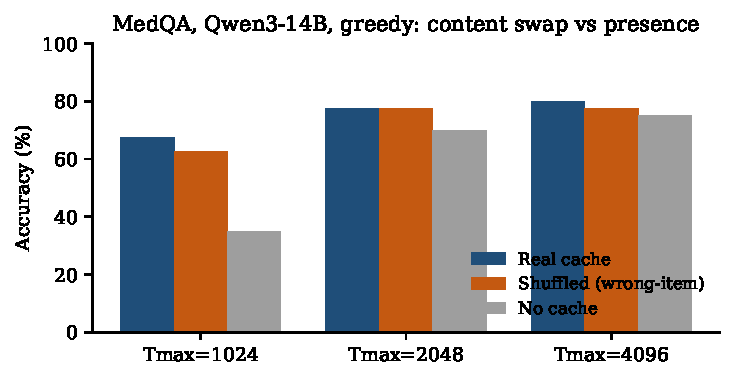
\includegraphics[width=\columnwidth]{figs/swap_budget.pdf}
\caption{Swap vs.\ presence on MedQA (greedy, $n{=}40$). A wrong-item cache
tracks the real cache; no cache hurts mainly when the Judger is short of
tokens.}
\label{fig:swap}
\end{figure}

\section{Most of a finished $K{=}40$ tape is droppable}
\label{sec:evict}

Table~\ref{tab:main} and Figure~\ref{fig:acc} report eviction under
\emph{their} sampling. Full $K{=}40$ vs.\ the same cache after eviction,
paired on the same items.

\begin{table}[t]
\centering
\small
\setlength{\tabcolsep}{2.4pt}
\begin{tabular}{lcccc}
\toprule
Task & $n{\times}$seeds & $K{=}40$ & Evict & Judger s \\
\midrule
GSM8K keep-64 & $100{\times}3$ & 96.3 & 95.7 & 14.4 / 13.0 \\
MATH-500 keep-128 & $100{\times}3$ & 85.7 & 83.7 & 34.2 / 31.8 \\
GPQA keep-128 & $100{\times}3$ & 53.7 & 48.7 & 87.6 / 65.8 \\
AIME24 keep-128 & $30{\times}3$ & 36.7 & 32.2 & 151 / 144 \\
AIME25 keep-128 & $30{\times}2$ & 35.0 & 31.7 & 155 / 144 \\
\bottomrule
\end{tabular}
\caption{Mean accuracy (\%) and mean Judger seconds (full / evict).
Relay storage is ${\sim}100$\,MB vs.\ $10$\,MB (GSM8K keep-64) or
$20$\,MB (keep-128). Upstream Planner/Critic/Refiner times match by
construction (${\approx}1$\,s each).}
\label{tab:main}
\end{table}

\begin{figure}[t]
\centering
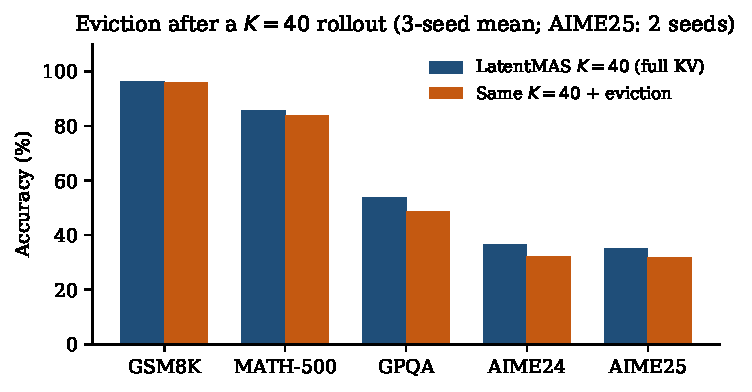
\includegraphics[width=\columnwidth]{figs/acc_evict.pdf}
\caption{Accuracy after deleting most KV slots of a $K{=}40$ relay.
Easy math holds; GPQA/AIME dip. This is a length ablation, not a new MAS.}
\label{fig:acc}
\end{figure}

\paragraph{Easy math.}
GSM8K is saturated either way. MATH-500 moves by two points. If the
uncompressed tape were a necessary workspace for the answer, keep-64/128
should not look like this.

\paragraph{Harder tasks.}
GPQA drops about five points; AIME about four, on $n{=}30$ where one
item is $3.3$ points. We do not spin a five-point GPQA dip into ``free
compression.'' We also do not need a collapse to conclude redundancy:
most of the tape can go and the system still answers in the same
ballpark.

\paragraph{The keep-16 knee.}
On GSM8K with the same $0.6/0.95$ protocol ($n{=}50$, seed 42), keep-16
ties full LatentMAS at $98\%$ accuracy but the Judger runs
\emph{longer} (${+}3$\,s, ${+}{\approx}120$ tokens). Deleting almost
everything preserves the answer and wrecks the short-CoT mode. The
scaffold is coarse, not empty.

\section{Eviction is not $K{=}10$}
\label{sec:notk10}

A reviewer can ask: why not set \texttt{latent\_steps=10}? That is a
different system. It never computes steps $11$--$40$. Eviction pays for
those steps, then throws most of them away. Table~\ref{tab:k10} is
therefore \emph{not} a claim that eviction wins. On GPQA, stopping at
$10$ is more accurate than our key-norm subset of a $K{=}40$ cache. The
row is here so the length-ablation is not misread as a hidden $K$-sweep.

\begin{table}[t]
\centering
\small
\begin{tabular}{lccc}
\toprule
Task & $K{=}40$ full & Evict & $K{=}10$ full \\
\midrule
GSM8K & 96.3 & 95.7 & 95.3 \\
MATH-500 & 85.7 & 83.7 & 83.7 \\
GPQA & 53.7 & 48.7 & 59.0 \\
AIME24 & 36.7 & 32.2 & 37.8 \\
\bottomrule
\end{tabular}
\caption{Early-stop ($K{=}10$) vs.\ select-from-$K{=}40$. Different
objects. $K{=}10$ is cheaper upstream (${\approx}0.27$\,s vs.\
${\approx}1.0$\,s per silent agent) and is \emph{not} our method.}
\label{tab:k10}
\end{table}

We do \emph{not} use Table~\ref{tab:k10} to contradict LatentMAS's
reported peak at $m{\approx}40$--$80$. That figure is a multi-point
sweep on their tasks and seeds. Two dots on GSM8K/MATH/GPQA, and
AIME where one problem is three points, are not that experiment.

\section{Systems side-effects, not the claim}
\label{sec:systems}

Figure~\ref{fig:lat} splits wall-clock. Eviction cannot reduce Planner,
Critic, or Refiner time: those forwards already happened. Judger time
moves when traces are long (GPQA: $88$\,s$\to 66$\,s) and barely moves
on GSM8K. Many AIME decodes hit an $8192$-token cap, so Judger time is
censored.

\begin{figure}[t]
\centering
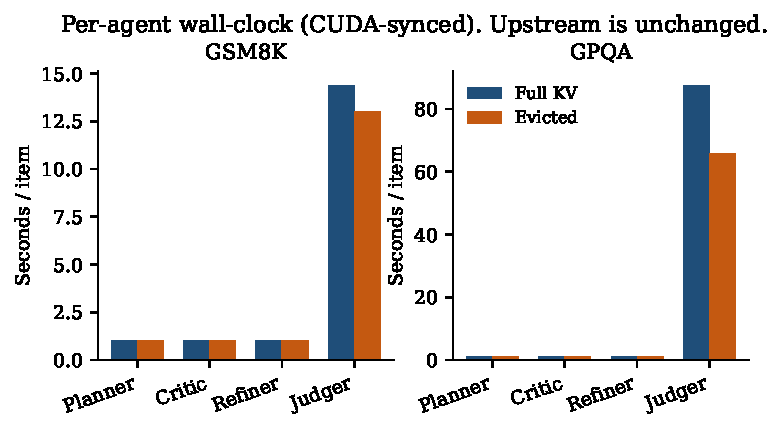
\includegraphics[width=\columnwidth]{figs/latency_agents.pdf}
\caption{CUDA-synced per-agent time. The silent agents are a fixed tax
at $K{=}40$; eviction only changes the Judger prefix.}
\label{fig:lat}
\end{figure}

Figure~\ref{fig:mem} is the batch-memory plot. Qwen3-14B weights are
${\approx}28$\,GB. One relay is ${\approx}100$\,MB vs.\ $10$\,MB after
keep-64. At Judger batch $B{=}64$ (short $16$-token decode, GSM8K donor
cache, H200), peak memory is $47$\,GB vs.\ $32$\,GB. Neither setting
OOM. Compression is a batched-KV saving, not an OOM rescue on this GPU
and not an accuracy result.

\begin{figure}[t]
\centering
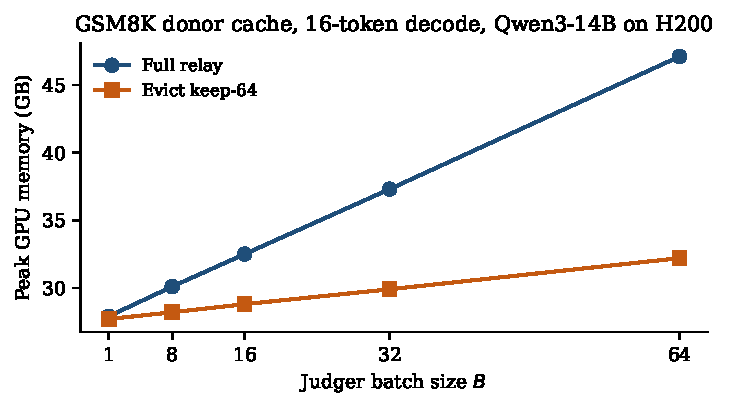
\includegraphics[width=\columnwidth]{figs/memory_batch.pdf}
\caption{Peak memory vs.\ Judger batch size. Weights dominate; the relay
is what scales with $B$.}
\label{fig:mem}
\end{figure}

\section{Related work}
\label{sec:related}

\paragraph{Latent and multi-agent reasoning.}
LatentMAS~\citep{zou2025latentmas} is the system we analyze.
Coconut~\citep{hao2024coconut} trains continuous latent thoughts inside
one model; we study a frozen multi-agent KV handoff, not a training
recipe. Text MAS~\citep{du2023society,wu2023autogen} exchanges language;
our question is whether replacing language with KV creates a message.

\paragraph{KV eviction.}
StreamingLLM attention sinks~\citep{xiao2024streamingllm} and
H2O heavy hitters~\citep{zhang2023h2o} motivate the heuristic. We use
them as a \emph{delete test} on an inter-agent relay, not as an
inference-engine contribution.

\paragraph{Analysis of internals.}
Probing, activation patching, and causal
interventions~\citep{belinkov2019analysis,meng2022rome,geva2023lm} are
the methodological family. Activation and KV
steering~\citep{turner2023actadd,rimsky2024caa,chen2025seal,li2025kvsteer}
supply the negative controls: the channel is hard to steer for
accuracy; the text-emitting Judger is not.

\section{Conclusion}
The $K{=}40$ LatentMAS relay behaves like a long prefix that induces a
Judger mode, not like a compact, instance-specific message. Swapping
content does little; deleting most positions of a finished tape does
little on easy math and only modestly more on GPQA. Naive eviction is
the delete test that makes that length claim checkable, plus a smaller
KV side-effect. The way to \emph{improve} latent MAS, if one wants a
methods paper, is to skip compute or replace the tape---not to celebrate
building forty steps and throwing them away.

\section*{Limitations}
One backbone (Qwen3-14B) and sequential LatentMAS only. Swap diagnostics
are greedy, smaller $n$, MedQA/GSM8K. Eviction uses a single importance
score; a better picker might keep more GPQA accuracy, which would
\emph{strengthen} the ``selection $\neq$ early-stop'' distinction rather
than the redundancy claim. AIME $n{=}30$ and frequent $8192$ caps limit
latency conclusions. LiveCodeBench was not run. We did not rerun
LatentMAS Figure~8. Eviction never reduces upstream FLOPs. Results are
analysis of one published system, not a universal theory of latent
communication.

\section*{Ethics statement}
This work analyzes a public multi-agent inference method on standard
academic benchmarks. It does not release new models or user data. The
main risk is over-interpreting a negative communication story as a
reason to deploy shorter, under-evaluated agent stacks.

% Bibliography
\bibliography{custom}

\appendix

\section{Fork check}
\label{app:fork}
\begin{table}[h]
\centering
\small
\begin{tabular}{lcc}
\toprule
Task ($K{=}40$, $n{=}150$, 1 seed) & Fork & Paper table \\
\midrule
GSM8K & 92.7 & 95.2 \\
ARC-Challenge & 94.7 & 95.6 \\
MedQA & 79.3 & 80.7 \\
\bottomrule
\end{tabular}
\caption{Functional check of the \texttt{9a9e4d3} fork vs.\ published
LatentMAS means (their 3-seed full sets). Gaps are consistent with
subset and seed, not a different algorithm.}
\end{table}

\section{Per-seed eviction accuracies}
\label{app:seeds}
GSM8K $K{=}40$/evict: $96/96$, $97/96$, $96/95$.
MATH-500: $86/86$, $86/84$, $85/81$.
GPQA: $52/48$, $52/44$, $57/54$.
AIME24: $37/37$, $37/27$, $37/33$ (percent, $n{=}30$).

\end{document}
